\documentclass[12pt,a4paper]{book}

\usepackage[italian]{babel}
\usepackage[utf8]{inputenc}
\usepackage[T1]{fontenc}
\usepackage{amsmath,amsfonts,amssymb,amsthm}
\usepackage{deistesi}
\usepackage{fancyhdr}

\usepackage[final]{listings}
\usepackage[table]{xcolor}

\definecolor{dkgreen}{rgb}{0.4,0.4,0.4}
\definecolor{gray}{rgb}{0.5,0.5,0.5}
\definecolor{dkgray}{rgb}{0.2,0.2,0.2}
\definecolor{commentgray}{rgb}{0.6,0.6,0.6}
\definecolor{mauve}{rgb}{0.58,0,0.82}

\lstset{
frame=single,
  captionpos=b,
  language=Python,
  aboveskip=3mm,
  belowskip=3mm,
  showstringspaces=false,
  columns=flexible,
  basicstyle={\fontsize{10}{10}\ttfamily},
  numbers=left,
  numberstyle=\tiny\color{gray},
  keywordstyle=\color{blue},
  commentstyle=\color{commentgray},
  stringstyle=\color{gray},
  breaklines=true,
  breakatwhitespace=true,
  tabsize=3,
  morekeywords={final},
  frame=single,
  rulecolor=\color{black}
}

\setlength{\textwidth}{13.5cm}
\setlength{\textheight}{19cm}
\setlength{\footskip}{3cm}
\setlength{\headheight}{15pt}
\oddsidemargin=50pt \evensidemargin=20pt

\titolo{ESLS: Esls Smart Light System}
\laureando{Ludovico de Nittis\\Eugenio Severi}
\annoaccademico{2016--2017}
\facolta{CAMPUS DI CESENA\\SCUOLA DI SCIENZE}
\corsodilaurea{Ingegneria e Scienze Informatiche}
\corso{\\Ingegneria dei Sistemi Software Adattativi Complessi\\Smart City}
%\relatore{.}
%\correlatorea[]{}
%\correlatoreb[]{Pablo Neruda}
\parolechiave{Bitcoin}{IoT}{Raspberry Pi}{Vending Machine}{Distributore Intelligente}
%\dedica{\textit{"Computers are like Old Testament gods; lots of rules and no mercy." - Joseph Campbell}}

\begin{document}

\frontmatter \maketitle \pagestyle{plain} \tableofcontents

\chapter{Introduzione}

Grazie alle potenzialità delle nuove tecnologie viviamo in un mondo sempre più connesso, aprendo la porta alle smart city e alle loro potenzialità.
Nell'ambito di questo progetto si è approfondito il tema dell'illuminazione pubblica, un servizio pervasivo sul territorio e che comporta notevoli costi per i comuni, specialmente per quanto riguarda la spesa per l'energia elettrica.
\\L'introduzione delle lampadine a led sta consentendo di ridurre notevolmente tali costi, ma ci si è chiesti se sia possibile contenerli ulteriormente attraverso ad un uso più efficiente nel tempo.
In particolare sono state osservate numerose inefficienze per quanto riguarda gli orari di accensione e spegnimento, spesso pianificati a priori con dei semplici timer, senza tenere conto del progressivo spostamento degli orari di alba e tramonto di ogni singolo giorno dell'anno e delle condizioni meteo che possono ridurre la visibilità (temporali, ecc.).
I timer vengono effettivamente regolati per periodi diversi dell'anno, ma non con il livello di granularità ottimale, in quanto per modificare gli orari impostati è necessario un intervento manuale di un addetto.
Inoltre, non tutte le zone di una città necessitano dello stesso livello di luminosità, sia a causa del differente utilizzo delle strade (strade principali, residenziali, del centro città, ecc.), sia a causa della specifica conformazione delle singole strade (ad esempio la presenza di alberi che ostacolano il passaggio della luce solare).
Infine, nelle ore notturne si può valutare una riduzione della normale luminosità dei lampioni, a causa del traffico estremamente ridotto.
\\Per questi motivi si è deciso di progettare e realizzare un sistema di gestione intelligente dell'illuminazione pubblica, consentendo una gestione remota dei lampioni (controllati da dispositivi embedded), di regolare automaticamente la loro intensità luminosa al variare delle condizioni ambientali e di monitorare il loro funzionamento in maniera centralizzata, al fine di consentire di prendere decisioni efficaci ai fini del risparmio energetico ma senza compromettere la qualità del servizio offerto.
\\La relazione è strutturata nei seguenti capitoli:
\begin{itemize}
 \item nel primo capitolo saranno definiti e analizzati i requisiti del sistema che si intende realizzare;
 \item nel secondo capitolo sarà descritta l'architettura del progetto, derivata dall'analisi dei requisiti, oltre allo schema di deployment;
 \item nel terzo capitolo verrà illustrata l'implementazione effettuata;
 \item nel quarto capitolo saranno presentati i test effettuati.
\end{itemize}


\mainmatter

% stile della pagina
\pagestyle{fancy} \fancyhead[LE,RO]{\bfseries\thepage}

% inclusione dei capitoli
\chapter{Stato dell'arte}

\section{Introduzione e cenni storici}


\chapter{Implementazione}

In questo capitolo verranno descritte le scelte implementative, derivate dalle scelte progettuali.

\section{Implementazione della parte server - Sistemistica}
In questa sezione verrà illustrata la configurazione software del server e dei suoi servizi.

\subsection{Server}
Per una maggiore chiarezza nell'esposizione, verrà considerato uno schema di deployment con un unico server sul quale sono in esecuzione tutti i servizi.
Nel caso di server multipli, quanto detto in seguito vale allo stesso modo: l'unica differenza saranno gli indirizzi IP diversi per ogni server.
Tutto il software utilizzato e sviluppato è pensato per funzionare correttamente sia in un ambiente distribuito che centralizzato.
Nell'ambito dello sviluppo di questo progetto, si è utilizzato un server virtuale fornito dal provider DigitalOcean con la seguente configurazione hardware:
\begin{itemize}
 \item 512 MB di RAM;
 \item 1 vCPU;
 \item 20 GB di memoria secondaria su SSD;
 \item 1 TB di traffico di rete massimo mensile.
\end{itemize}
Una configurazione di questo tipo, seppure minimale, è più che adatta allo sviluppo e a piccole installazioni; per gestire sistemi di più grandi dimensioni si suggerisce una dotazione hardware più performante.
Ad ogni modo, come evidenziato in fase di progettazione, nel caso di installazioni di grandi dimensioni, si sconsiglia l'utilizzo di un unico server ad alte performance in favore di un cluster di più server individualmente meno potenti, al fine di garantire ridondanza.

\subsection{Sistema operativo, impostazioni e servizi di sistema}
Valutati i sistemi operativi presenti sul mercato, si è scelto di utilizzare una distribuzione Linux per i seguenti motivi:
\begin{itemize}
 \item coerenza con gli altri componenti del sistema;
 \item sistema operativo open source, quindi tendenzialmente più sicuro;
 \item possibilità di evitare costi di licenza, grazie alla licenza GNU-GPL.
\end{itemize}
In particolare, è stata utilizzata la distribuzione Ubuntu Server 16.04, basata sul kernel Linux 4.4, in quanto è una delle distribuzioni maggiormente diffuse in ambito server, è ben documentata, e utilizza software mediamente più aggiornato rispetto ad altre distribuzioni come Debian o CentOS.
Il software utilizzato è comunque disponibile per tutte le principali distribuzioni, quindi la scelta è in realtà libera, in base alle necessità delle singole installazioni.
Per motivi di sicurezza, è fondamentale aggiornare regolarmente i software installati per far fronte alle nuove vulnerabilità.
Questa operazione può essere eseguita manualmente da un sistemista, oppure pianificata automaticamente (nel caso di Ubuntu, configurando il pacchetto \textit{unattended-upgrades}).
\\Le seguenti funzionalità e servizi di sistema sono stati installati e configurati.
\paragraph{Utenti}
Per motivi di sicurezza è opportuno creare per ogni amministratore del server un utente distinto con privilegi ridotti.
Le operazioni che richiedono privilegi elevati devono essere eseguite utilizzando il comando \textit{sudo}, e mai autenticandosi direttamente come \textit{root}.
Ogni servizio in esecuzione dovrebbe idealmente essere eseguito utilizzando un account utente ad hoc dotato dei soli privilegi necessari all'esecuzione di quello specifico servizio.
\paragraph{AppArmor}
Come misura di sicurezza aggiuntiva, per limitare gli eventuali danni nel caso si verificasse un'intrusione, in aggiunta al Discretionary Access Control utilizzato da Linux, è buona norma utilizzare un meccanismo di Mandatory Access Control per confinare quanto più possibile ogni singolo processo.
Nell'ambito di questa installazione è stato utilizzato AppArmor. In alternativa, è possibile utilizzare SELinux, che fornisce un livello di granularità maggiore, ma è anche notevolmente più complesso da configurare.
Data la natura del servizio, tale per cui solo un amministratore è in grado di aprire una shell sul server, e non essendo i dati trattati critici, AppArmor è più che adeguato allo scopo.
\paragraph{SSH}
Il servizio SSH (Secure Shell) è utilizzato esclusivamente dall'amministratore per eseguire operazioni di manutenzione sul server.
Rispetto alla configurazione di default, sono state aggiunte alcune impostazioni di hardening, in quanto si tratta del servizio più appetibile per un eventuale attaccante: una compromissione di SSH consentirebbe di eseguire comandi dannosi, e aprirebbe la porta allo sfruttamento di vulnerabilità che potrebbero portare ad una privilege escalation a root, compromettendo l'intero server.
Le impostazioni aggiuntive di OpenSSH server sono:
\begin{itemize}
 \item consentire solo la versione 2 del protocollo SSH (la 1 è insicura);
 \item abilitazione dei soli algorigmi crittografici di scambio chiavi considerati robusti (\textit{curve25519-sha256@libssh.org,diffie-hellman-group-exchange-sha256}), disabilitando quelli meno sicuri (presenti per retrocompatibilità);
 \item disabilitazione dei moduli per lo scambio chiavi Diffie-Hellman con chiave più corta di 2048 bit;
 \item utilizzare chiavi private per il server di adeguata lunghezza e solo con algoritmi sicuri (\textit{ed25519,rsa});
 \item impedire l'autenticazione dei client tramite password, ma solo tramite chiavi asimmetriche (\textit{PasswordAuthentication no; ChallengeResponseAuthentication no; PubkeyAuthentication yes});
 \item abilitazione dei soli algoritmi di crittografia simmetrica considerati robusti (\textit{chacha20-poly1305@openssh.com,aes256-gcm@openssh.com,aes128-gcm@openssh.com,aes256-ctr,aes192-ctr,aes128-ctr}), disabilitando quelli meno sicuri (presenti per retrocompatibilità);
 \item abilitazione dei soli algorigmi MAC (Message Authentication Code) considerati robusti (\textit{hmac-sha2-512-etm@openssh.com,hmac-sha2-256-etm@openssh.com,hmac-ripemd160-etm@openssh.com,umac-128-etm@openssh.com,hmac-sha2-512,hmac-sha2-256,hmac-ripemd160,umac-128@openssh.com}), disabilitando quelli meno sicuri (presenti per retrocompatibilità);
 \item nel caso lo si ritenesse opportuno, è possibile implementare una forma di autenticazione a due fattori sfruttando un modulo PAM (Pluggable Authentication Module).
\end{itemize}
\paragraph{Fail2Ban}
Al fine di prevenire attacchi di tipo brute-force o basati su dizionario, può essere opportuno utilizzare \textit{Fail2Ban}, un demone che controlla nei file di log la presenza di tentativi di accesso non riusciti e di bloccare temporaneamente gli indirizzi IP dai quali provengono.
Per evitare che anche gli utenti legittimi vengano bloccati accidentalmente, è buona norma consentire un certo numero di tentativi prima di attuare il blocco.
Qualora l'indirizzo IP di un utente legittimo venisse bloccato, per tentare nuovamente di accedere è necessario attendere la scadenza del blocco o di accedere direttamente alla console del server.
\paragraph{UFW}
Essendo il sistema in rete, è necessario configurare il firewall per limitare il traffico ai soli servizi necessari. In questa implementazione è stato utilizzato \textit{UFW}, ma è possibile utilizzare anche \textit{iptables}.
Innanzitutto devono essere bloccate tutte le connessioni in ingresso ad eccezione di quelle necessarie al funzionamento del servizio. Quali siano effettivamente necessarie dipende dall'architettura di deployment (server singolo o più server) e dall'eventuale utilizzo di VPN.
Nel caso più semplice (tutti i servizi su uno stesso server), è necessario esporre verso l'esterno solamente SSH, il server web per la gestione e il sistema di generazione di grafici e statistiche.
Nel caso tutta la rete dei Raspberry fosse contenuta in una VPN o in una rete locale, si potrebbe esporre i singoli servizi solo sulle interfacce deputate a fornire quello specifico servizio.
In generale, il livello di isolamento sarà direttamente proporzionale alla sicurezza della rete.
Tuttavia, essendo tutte le informazioni in transito crittografate, il transito delle informazioni su rete pubblica non dovrebbe costituire un problema (salvo eventuali vulnerabilità scoperte in seguito nei software).
Anche nel caso il sistema trasmetta su una rete pubblica, qualora sia stata acquistata una sottorete di indirizzi IP pubblici, è consigliabile consentire connessioni solo da e verso gli indirizzi di quella sottorete.

\subsection{Server Web}
Il server web utilizzato per ospitare l'interfaccia di gestione dei Raspberry è \textit{nginx}. È stato scelto per:
\begin{itemize}
 \item la sua leggerezza;
 \item le elevate prestazioni;
 \item la scalabilità.
\end{itemize}
Allo stato attuale il carico su questo servizio si mantiene basso, in quanto le richieste che deve gestire sono poche contemporaneamente (solo gli operatori manutentori accedono a questo servizio).
Di conseguenza, è possibile utilizzare anche altri server web, ad esempio Apache. L'utilizzo di \textit{nginx} è stato pensato per far fronte ad eventuali nuove funzionalità future.
Come misura di sicurezza, tutte le connessioni sono protette tramite TLS 1.2, per evitare intercettazioni ed attacchi di tipo man-in-the-middle.
I dettagli implementativi dell'interfaccia web per controllare i Raspberry sono indicati in seguito nella sezione \ref{serv-rest-in}.

\subsection{Time Series DBMS \label{tsdbms}}
Come evidenziato in fase di progettazione, l'utilizzo di un Time Series database è particolarmente indicato per l'archiviazione dei dati statistici prodotti dai Raspberry.
Si è scelto di installare InfluxDB, un TS-DBMS open source sviluppato da InfluxData, scritto in \textit{Go} e ottimizzato per l'archiviazione di dati ad alte prestazioni, per la ricerca efficiente su serie di dati, e con supporto all'alta disponibilità.
La modalità principale di accesso ai dati è tramite un'interfaccia REST, in linea con i requisiti del sistema, sebbene esistano librerie per l'utilizzo con vari linguaggi di programmazione.
Nel caso di installazioni più piccole, sarebbe pensabile anche l'utilizzo di un DBMS relazionale, ma si rivelerebbe una scelta poco scalabile.
I dati vengono inviati ad InfluxDB esclusivamente dalle istanze della servlet, che fungono da mediatori tra i Raspberry e il database.
Sono stati implementati tre tipi di messaggi archiviabili sul database: \textit{changeLightIntensity}, \textit{changePolicy}, \textit{notifyError}.
\paragraph{Messaggio ``changeLightIntensity''}
Questo messaggio viene generato ogni qual volta un Raspberry modifichi l'intensità luminosa dei lampioni ad esso collegati e contiene i seguenti campi:
\begin{itemize}
 \item un riferimento all'host che ha generato l'evento;
 \item l'azione eseguita (accensione, spegnimento, variazione di luminosità dovuta a politiche di risparmio energetico o al passaggio di un'auto);
 \item un riferimento alla zona/gruppo in cui il Raspberry si trova;
 \item l'intensità luminosa impostata;
 \item l'intensità di luce ambientale rilevata;
 \item un timestamp relativo al momento della generazione dell'evento.
\end{itemize}
\paragraph{Messaggio ``changePolicy''}
Questo messaggio viene generato quando vengono modificate le policy di un lampione (orari di accensione e spegnimento e soglie di luminosità.
In questo caso vengono registrati i seguenti parametri:
\begin{itemize}
 \item un riferimento all'host che ha generato l'evento;
 \item un riferimento alla zona/gruppo in cui il Raspberry si trova;
 \item un timestamp relativo al momento della generazione dell'evento.
\end{itemize}
\paragraph{Messaggio ``notifyError''}
Questo messaggio viene generato quando un Raspberry auto-diagnostica un errore interno e ha lo scopo di avvisare l'amministratore che è necessario un intervento manuale.

\subsection{Sistema di generazione di statistiche e grafici}
Per analizzare in maniera proficua la grande quantità di dati potenzialmente archiviata del database InfluxDB si è scelto di utilizzare il software \textit{Grafana}, software specializzato nella generazione di grafici statistici basati sui dati contenuti in TS-DBMS.
La scelta è ricaduta su questo strumento specifico in quanto è estremamente flessibile, consentendo agli amministratori di generare i grafici di loro interesse filtrando e aggregando i dati.
In questo modo gli amministratori possono creare dinamicamente i grafici di cui hanno bisogno, adattandosi in questo modo sia alla topologia della città in cui il sistema è installato, sia alle necessità specigiche che potrebbero sorgere in maniera imprevedibile (ad esempio potrebbe sopraggiungere la necessità di monitorare con maggiore granularità un'area della città in particolare, qualora si rilevasse un numero di guasti fuori norma).
Gli amministratori potranno quindi creare alcuni grafici di interesse generale sempre disponibili e altri dinamicamente in base alle necessità, in maniera simile a quello che avviene nella navigazione di un data-warehouse, ma orientato alle serie di dati.
I grafici sono creabili e consultabili utilizzando l'interfaccia web di Grafana. Qualora si rendesse necessario creare grafici estremamente personalizzati, è anche possibile scrivere direttamente le query per interrogare il database.
Per il rilevamento di guasti, si possono generare grafici che mettono in risalto comportamenti al di fuori della media (lampioni che si accendono in orari completamente diversi dagli altri, Raspberry che improvvisamente smettono di inviare dati, ecc.).
% TODO inserire uno screen di grafana

\subsection{DBMS relazionale}
Opzionalmente, si può valutare di utilizzare un database relazionale di supporto per memorizzare:
\begin{itemize}
 \item l'anagrafica dei Raspberry dislocati sul territorio;
 \item le credenziali di accesso ai singoli Raspberry;
 \item eventuali dati statistici sintetici relativi allo storico dei guasti.
\end{itemize}
% TODO Da rivedere


\section{Implementazione della servlet \label{serv-impl}}
Come descritto nell'architettura nel capitolo precedente, i dispositivi Raspberry non comunicano direttamente con il database, ma si affidano ad una o più istanze di una servlet intermediaria.
Il linguaggio di programmazione scelto per l'implementazione è Java, poiché è disponibile per un'ampia varietà di sistemi operativi ed esiste un ampio supporto da parte di librerie esterne.
Data la natura dell'applicazione, che necessita di reattività e scalabilità, l'implementazione è stata realizzata sfruttando \textit{Vert.x}, una libreria integrabile in Java che consente di utilizzare un paradigma event-driven e non bloccante, particolarmente indicata per la realizzazione di microservizi REST.
Resta comunque possibile implementare la servlet con altre tecnologie e linguaggi di programmazione, a patto di mantenere invariate le interfacce REST.

\subsection{Interfaccia REST in ingresso \label{serv-rest-in}}
La servlet viene contattata dai Raspberry (client) con un messaggio JSON contenente una serie di dati, dipendente dal tipo di messaggio. Tutte le connessioni crittografate e autenticate con TLS.
I possibili campi sono:
\begin{itemize}
 \item "area": campo numerico che corrisponde alla zona di appartenenza del lampione. Serve a fini statistici per aggregare i dati;
 \item "action": campo che corrisponde al tipo di azione che è stata eseguita, e può essere uno tra: \textit{turn\_on}, \textit{turn\_off}, \textit{energy\_saving} o \textit{car\_detected};
 \item "intensity": campo numerico relativo all'intensità di luce attuale del lampione;
 \item "photoresistor": campo numerico relativo alla lettura della fotoresistenza;
 \item "timestamp": campo che contiene il timestamp in cui è avvenuta l'azione.
\end{itemize}

\subsection{Interfaccia REST in uscita}
La servlet, nel suo ruolo di mediatore, esegue la conversione dei dati JSON ricevuti dai Raspberry nel formato richiesto dal database, e lo contatta utilizzando a sua volta un'interfaccia REST (in questo caso la servlet si comporta da client rispetto al database (server)).
Il contenuto dei messaggi è descritto nella parte di dettaglio del Time Series Database (sezione \ref{serv-rest-in}).
Per motivi di sicurezza, ad ogni risposta ai client, vengono inseriti alcuni header HTTP per mitigare l'impatto di vulnerabilità Cross Site Scripting (XSS) e altri usi scorretti, oltre a disabilitare il caching (non necessario in questo tipo di applicazione).

\subsection{Parametri della servlet}
Se avviata senza specificare alcun parametro, la servlet utilizzerà quelli di default; è altrimenti possibile specificarli tramite argomenti dalla linea di comando. I parametri sono:
\begin{itemize}
 \item \textit{dbhost}: indirizzo IP del database (di default 127.0.0.1);
 \item \textit{listenPort}: porta TCP sulla quale la servlet è in ascolto (di default 44343);
 \item \textit{dbPort}: porta TCP sulla quale il TS-DBMS è in ascolto (di default 8086);
 \item \textit{dbName}: nome del database sul server TS-DBMS (di default ``esls'').
\end{itemize}
Altri parametri hard-coded sono:
\begin{itemize}
 \item \textit{API\_LEVEL}: numero di versione dell'interfaccia REST (inviato dai Raspberry ad ogni richiesta REST, utile per mantenere retrocompatiblità con eventuali nuove versioni della servlet e del software su Raspberry);
 \item \textit{BODY\_SIZE\_LIMIT}: limita la dimensione del buffer per le richieste HTTP in ingresso (utile per mitigare gli attacchi DDoS)
\end{itemize}


\section{Implementazione della parte embedded - Raspberry}
In questa sezione verrà illustrata l'implementazione della parte Raspberry.

\subsection{Hardware}
%TODO
\paragraph{Raspberry Pi}
%TODO dotazione hardware raspberry
\paragraph{Sensori e attuatori}
%TODO sensori e attuatori utilizzati

\subsection{Sistema operativo e servizi di sistema}
Per quanto riguarda la scelta del sistema operativo da utilizzare, la scelta è ricaduta sulla distribuzione Linux Raspbian, in quanto è la principale distribuzione ufficialmente supportata per Raspberry e, basandosi su Debian, offre un livelli di leggerezza, stabilità e sicurezza elevati.
Queste caratteristiche sono di grande importanza in un sistema di questo tipo, ovvero in cui i Raspberry sono dislocati sul territorio e collegati in rete.
Ad ogni modo, sebbene la scelta della distribuzione sia ricaduta su Raspbian, è possibile utilizzare una qualsiasi altra distribuzione Linux semplicemente installando tutte le dipendenze necessarie che verranno utilizzane in fase di implementazione del progetto.
\paragraph{Nota sulla gestione del tempo}
I messaggi che i Raspberry Pi inviano quando comunicano con il server contengono al loro interno anche un timestamp per fini statistici.
Per evitare che col passare del tempo l'orario vada fuori sincrono, si è impostato l'aggiornamento tramite server \textit{NTP} su base giornaliera invece che, come di default, ad ogni avvio: i Raspberry possono restare attivi per lunghi periodi senza essere riavviati.
\paragraph{SSH}
%TODO (vedere anche la mia sezione su ssh più in alto in questo capitolo per i concetti di base. Però più sintetica)

\subsection{Linguaggio di programmazione, paradigma ad attori e organizzazione a task}
Per il programma in esecuzione sui Raspberry Pi si è scelto di utilizzare Python 3, che garantisce un elevato supporto per i sensori e attuatori attualmente disponibili.
%TODO Aggiungere qualcosa per tessere le lodi di Python (perché proprio Python e non C/Java/qualunque altra cosa?)
Essendo il software dei Raspberry composto da diverse parti tra loro autonome e concorrenti, si è scelto di utilizzare il paradigma ad attori (tramite la libreria \textit{Pykka}), un modello computazione concorrente a più alto livello rispetto alla gestione manuale dei thread, in quanto si addice maggiormente alla struttura interna del progetto.
In questo modo ogni componente logica è un attore e la comunicazione avviene esclusivamente tramite scambio di messaggi. In risposta ad un messaggio ricevuto un attore può:
\begin{itemize}
 \item prendere una decisione locale;
 \item creare nuovi attori;
 \item inviare nuovi messaggi;
 \item determinare come rispondere al successivo messaggio che potrà ricevere.
\end{itemize}
Come definito in fase di progettazione, i Raspberry devono poter eseguire diverse operazioni concorrentemente, tra cui:
\begin{itemize}
 \item rimanere in ascolto per eventuali richieste REST;
 \item controllo della presenza di auto;
 \item rilevamento dell'intensità luminosa;
 \item gestione dell'illuminazione dei lampioni in base ad uno scheduling.
\end{itemize}
La libreria \textit{threading} di Python, che permette ad un singolo programma l'esecuzione di più thread, è stata impiegata.

\subsection{Controllo presenza auto \label{cpa}}
Per controllare la presenza di auto sulla carreggiata viene effettuato il calcolo della distanza utilizzando il sensore ad ultrasuoni HC-SR04.
Per mitigare eventuali errori grossolani vengono effettuate sempre due misurazioni, calcolando successivamente la media.
La misurazione avviene inviando un segnale ad ultrasuoni e calcolando il tempo che il segnale impiega per andare e tornare, rimbalzando sugli oggetti.
Per calcolare la distanza in centimetri si moltiplica il tempo per la velocità del suono nell'aria (34300 cm/s) e il tutto viene diviso per 2 (perché il tempo era relativo all'andata e ritorno).
Per capire la direzione di marcia di un auto, nel caso di strade a doppio senso di marcia, è possibile adottare due strategie.
\begin{itemize}
 \item Posizionare nelle vicinanze del primo e dell'ultimo lampione, controllati da un determinato Raspberry, una coppia di sensori ad ultrasuoni a qualche centimetro di distanza tra loro: in questo modo controllando in quale sequenza la coppia di sensori rileva la presenza di un auto è possibile intuirne la direzione di marcia.
 \item Posizionare in tutto due sensori ad ultrasuoni vicino ai lampioni controllati da un determinato Raspberry: il primo andrà posizionato vicino al primo lampione sullo stesso lato della strada, e il secondo andrà vicino all'ultimo lampione sul lato opposto della strada.
 In questo modo impostando una soglia per il rilevamento delle auto pari al limite delle due carreggiate sarà possibile valutare il senso di marcia delle auto.
 Quindi, se per esempio il limite della carreggiata si trova a due metri dal bordo della strada, si imposterà il sensore in modo che se rilevi solo oggetti distanti meno di due metri, ed essi verranno considerati auto in transito sulla propria carreggiata.
\end{itemize}
Per l'implementazione di questo progetto si è optato per l'utilizzo della seconda strategia perché consente di ottenere lo stesso risultato utilizzando solo due sensori ad ultrasuoni invece che quattro, contenendo i costi.
L'utilizzo della prima strategia potrebbe tornare utile nel caso si voglia calcolare anche la velocità di crociera dei veicoli in transito.
In questo progetto essere in grado di capire il senso di marcia permette di accendere i lampioni in sequenza seguendo il verso di percorrenza.
Il thread che si occupa del sensore di prossimità utilizza un secondo thread per inviare il segnale ad ultrasuoni.
Grazie a questa scelta si evita che il thread principale del sensore vada in busy waiting attendendo l'invio e il ritorno del segnale ad ultrasuoni.
Inoltre si è utilizzata la funzione \textit{wait\_for\_edge} che permette di fermare l'esecuzione del thread fino a quando non viene rilevata un'oscillazione, consumando una quantità minima di CPU.
Per impostazione predefinita, il processo di misurazione considera la presenza di un veicolo sulla strada se la distanza rilevata è minore di due metri.
Tale valore può essere facilmente regolato in base alle caratteristiche della strada in cui si intende installare i sensori.
Il processo di controllo presenza auto è rappresentato da un attore il quale, dopo aver effettuato un controllo, notifica tutti i lampioni interessati.

\newpage
\lstinputlisting{code/ultrasonic.py}

\subsection{Rilevamento intensità luminosa}
Considerando che il Raspberry Pi non dispone di PIN analogici, per effettuare le letture di luminosità è possibile utilizzare le seguenti modalità:
\begin{itemize}
 \item collegare un altro controllore che abbia pin analogici (ad esempio Arduino) e utilizzare una fotoresistenza analogica;
 \item utilizzare una fotoresistenza analogica collegandola ad un convertitore analogico-digitale (ADC);
 \item utilizzare un sensore di luminosità digitale.
\end{itemize}
La prima modalità potrebbe essere presa in considerazione nel caso in cui si debba utilizzare diversi tipi di sensori analogici, tali da giustificare l'utilizzo di un controllore esterno, che comporterebbe maggiori costi e introdurrebbe complessità nel sistema.
Anche la seconda modalità può essere utile se si deve utilizzare più di un sensore analogico visto che un singolo ADC permette di utilizzare diversi pin analogici, ma è conveniente rispetto alla prima, in quanto più economica e non introduce particolare complessità.
In questo caso, dovendo collegare una singola fotoresistenza, si è optato per la terza modalità, utilizzando il sensore digitale TSL2561.
In alternativa si potrebbe prevedere l'utilizzo di più sensori di luminosità in modo da essere in grado di effettuare una media delle letture, compensando eventuali letture errate dovute ad eventuali danneggiamenti o residui di sporco che potrebbero coprire il sensore.
Come per il controllo di presenza di auto della sezione \ref{cpa}, anche il processo di rilevamento è gestito da un attore.

\subsection{Scheduling illuminazione \label{si}}
%TODO questa sezione è lunga e poco strutturata. Valutare di spezzarla in più paragraph o, se complicasse troppo la formattazione, al limite di andare a capo quando si cambia argomento
Per quanto riguarda la programmazione dell'illuminazione, il sistema offre la possibilità di impostare su base giornaliera un orario di accensione, di spegnimento, di inizio e di fine del periodo di risparmio energetico.
% in fase di progettazione è stato spiegato cos'è il periodo di risparmio energetico?
In tutte e quattro le impostazioni, oltre all'orario, è previsto anche un campo relativo alla soglia di intensità luminosa desiderata.
Come scelta implementativa, si è deciso di dare la precedenza alla luminosità rilevata rispetto all'orario.
Di conseguenza il funzionamento sarà il seguente: supponiamo di aver programmato l'accensione dei lampioni per le 19:00 con un livello di luminosità nell'ambiente pari a 50.
Se alle 19:00 l'intensità luminosa rilevata fosse minore di 50, i lampioni si accenderebbero; nel caso in cui l'intensità luminosa fosse maggiore di 50 i lampioni rimarrebbero spenti nonostante siano le 19:00.
È stata effettuata questa scelta perché se la luminosità esterna rilevata fosse alta sarebbe poco sensato accendere anche i lampioni.
Al contrario, se la luminosità rilevata fosse bassa, questo potrebbe anche essere dovuto a residui di sporco che con il tempo potrebbero depositarsi sul sensore.
Quindi anche se si rileva un livello di luminosità basso, si aspetta comunque l'orario impostato per accendere i lampioni.
La programmazione temporale viene espressa con precisione al minuto, visto che considerare anche i secondi comporterebbe un livello di precisione inutilmente elevato per questo scenario applicativo.
La configurazione dei lampioni potrebbe essere salvata:
\begin{itemize}
 \item in locale su ogni dispositivo embedded o su un server centralizzato;
 \item utilizzando un database relazionale o un file di testo.
\end{itemize}
Salvando le configurazioni su un server centrale si avrebbe il vantaggio di poter effettuare query consultando un singolo server e di gestire facilmente il backup centralizzato delle configurazioni;
d'altro canto, ogni dispositivo embedded dovrebbe sempre contattare il server per poter venire a conoscenza della propria programmazione e, nel caso in cui la connessione ad internet venisse a mancare, il dispositivo embedded smetterebbe di funzionare.
Salvando le configurazioni in locale su ogni Raspberry si ha una maggiore resistenza ai guasti visto che, anche nel caso in cui la connessione internet venisse persa, il dispositivo embedded potrebbe continuare a funzionare essendo il proprio comportamento totalmente locale.
Un database relazionale potenzialmente potrebbe offrire prestazioni maggiori rispetto ad un file di testo, ma tale vantaggio sarebbe evidente solo nel caso in cui i dati da salvare fossero in numero considerevole, e non è questo il caso;
un file di testo con una certa sintassi permette di controllare i valori salvati e di modificarli anche manualmente agendo direttamente sul file senza effettuare complicate query SQL.
Considerando i requisiti di progettazione come l'affidabilità del sistema e la facilità di gestione, si è scelto di salvare le configurazioni utilizzando un file di testo locale su ogni dispositivo embedded.
Inoltre il deploy dei dispositivi embedded potrebbe essere automatizzato, ad esempio tramite l'utilizzo di software quali \textit{Ansible} o \textit{Puppet}.
Grazie a questa scelta gli addetti ai lavori possono effettuare una programmazione agevole su ogni singolo lampione sia tramite interfaccia web che direttamente modificando i file di testo (tramite SSH o localmente).
Per il formato con cui vengono salvate le configurazioni si è scelto di utilizzare il \textit{Configuration file parser} presente nelle librerie standard di Python, perché permette la creazione di configurazioni con un linguaggio semplice, con una struttura simile ai file \textit{INI} di Microsoft Windows.
Questo garantisce una facile lettura e modifica anche manuale dei file. I file così creati hanno una estensione \textit{cfg}. I file hanno quattro sezioni principali con diversi campi ciascuna.
La prima sezione è \textit{GENERAL} e prevede tre campi:
\begin{itemize}
 \item \textit{lamp\_id}: un identificativo intero progressivo del singolo lampione;
 \item \textit{lamp\_pin}: il numero del pin a cui il lampione è collegato sul dispositivo embedded;
 \item \textit{lamp\_area}: la zona di appartenenza del singolo lampione.
\end{itemize}
La seconda sezione \textit{LampPolicyOn} e la terza \textit{LampPolicyOff} hanno gli stessi campi:
\begin{itemize}
 \item \textit{intensity}: l'intensità di luce del lampione espressa con un numero da 0 a 100 (impostare l'intensità a 0 equivale a spegnere il lampione);
 \item \textit{time\_h}: l'ora a cui questa impostazione dovrà iniziare;
 \item \textit{time\_m}: il minuto a cui questa impostazione dovrà iniziare;
 \item \textit{photoresistor}: la soglia richiesta di luminosità ambientale.
\end{itemize}
La quarta sezione è \textit{LampEnergySaving} e prevede cinque campi:
\begin{itemize}
 \item \textit{intensity}: l'intensità di luce del lampione espressa con un numero da 0 a 100;
 \item \textit{time\_h\_on} e \textit{time\_m\_on}: rispettivamente l'ora e i minuti in cui inizia la modalità risparmio energetico;
 \item \textit{time\_h\_on} e \textit{time\_m\_on}: rispettivamente l'ora e i minuti in cui termina la modalità risparmio energetico.
\end{itemize}
Per una questione di coerenza l'inizio e la fine della modalità risparmio energetico deve essere obbligatoriamente compresa tra \textit{LampPolicyOn} e \textit{LampPolicyOff}.
In definitiva grazie a tale implementazione si è reso possibile sia la modifica dello scheduling di un singolo lampione con la comodità della interfaccia web, sia una modifica più avanzata collegandosi per esempio in SSH ad un Raspberry e cambiando i valori manualmente sui file di configurazione.

\lstinputlisting{code/light0.cfg}
\newpage

\subsection{Messaggi a fini statistici}
Quando i dispositivi embedded eseguono azioni rilevanti, inviano ad un'istanza della servlet (sezione \ref{serv-impl}) un messaggio \textit{JSON} per consentire agli addetti ai lavori di avere una panoramica generale sull'andamento dell'intero sistema.
I possibili campi del messaggio sono stati descritti nella sezione \ref{serv-rest-in} relativa all'implementazione della servlet.

\subsection{API REST}
Come scritto in fase di progettazione, i Raspberry Pi devono esporre un insieme di API di tipo REST per consentire la modifica delle policy relative alla programmazione dei lampioni.
Per tale scopo è stata utilizzata la libreria \textit{Flask}.
Quando un Raspberry riceve una richiesta tramite la API REST, per prima cosa vengono controllate le credenziali fornite, in quanto è sempre richiesta un'autenticazione tramite username e password per poter completare una qualsiasi operazione GET o POST.
Nel caso la richiesta ricevuta sia valida, verrà restituito un JSON contenente o i dati richiesti, o il codice di stato HTTP 200 (nel caso in cui la richiesta non preveda dati di ritorno) per confermare la riuscita dell'operazione.
%da rivedere e espandere

\subsection{Modalità Debug}
Per consentire agli addetti ai lavori di effettuare controlli sui lampioni, come per esempio verificare il loro corretto funzionamento, è stata prevista la possibilità di abilitare la modalità debug.
Entrando in modalità debug i lampioni si accenderanno e spegneranno in base ai comandi che verranno impartiti manualmente, ignorando le eventuali policy impostate in precedenza.
Per abilitarla è necessario inviare una richiesta POST all'indirizzo \textit{/debug/lamp/<int:lamp\_id>/on} (per accendere un lampione) oppure a \textit{/debug/lamp/<int:lamp\_id>/off} (per spegnere un lampione).
Le richieste POST dovranno contenere un campo \textit{intensity} che corrisponde all'intensità luminosa desiderata a cui si intende impostare il lampione.
Quando si vuole concludere la fase di debug bisogna inviare una POST all'indirizzo \textit{/debug/lamp/<int:lamp\_id>/stop}.
Una volta conclusa la fase di debug, i lampioni torneranno a funzionare seguendo il proprio scheduling.

\subsection{Gestione dei guasti}
%TODO: cosa succede se un rasp si rompe? Cosa continua a funzionare e cosa no a seconda del tipo di guasto (guasto di rete, hardware, ...). Parlare anche della notifica del guasto al server (ipotizzando di avere hardware che si accorge dei led bruciati, che però nella nostra implementazione non c'è, ma il software deve supportarlo).

\section{Implementazione dell'interfaccia Web di manutenzione}
Come illustrato nella sezione \ref{si}, per permettere agli addetti ai lavori di controllare e modificare la programmazione dei singoli lampioni è stata implementata un'interfaccia Web tramite un server REST.
Come misura di sicurezza, tutte le richieste GET e POST ai Raspberry dovranno essere corredate da nome utente e password relativi al singolo dispositivo embedded che si intende contattare.
%(mmm, la storia del "dare ad un addetto solo le credenziali dei rpi della sua zona dove lo mettiamo?) --> nella sezione DBMS relazionale. Ma al momento non è implementato, quindi aspetto a scriverlo.
Il sito Web è stato realizzato seguendo uno stile minimale, moderno e il quanto più intuitivo per l'utente.
L'interfaccia è ottimizzata sia per un uso desktop che mobile.
\begin{figure}[tbp]
	\centering
	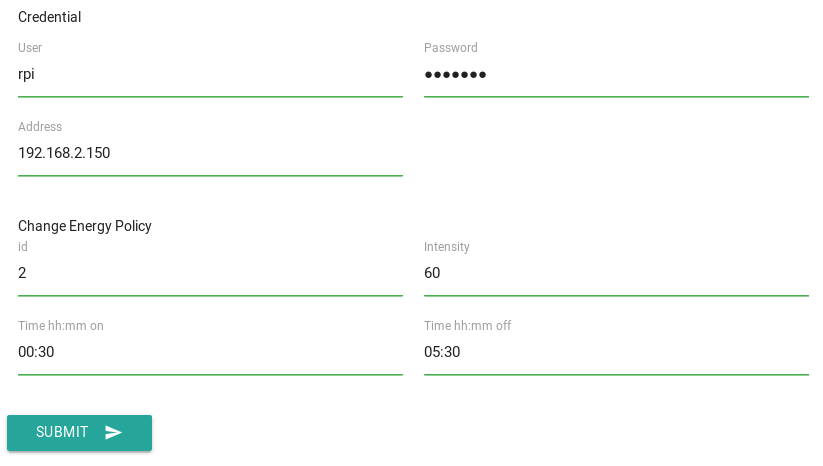
\includegraphics[scale=.62]{figure/web_desktop.png}
	\caption{Interfaccia web Desktop \label{WD}}
	\subfloat[(Mobile) Campi corretti]{{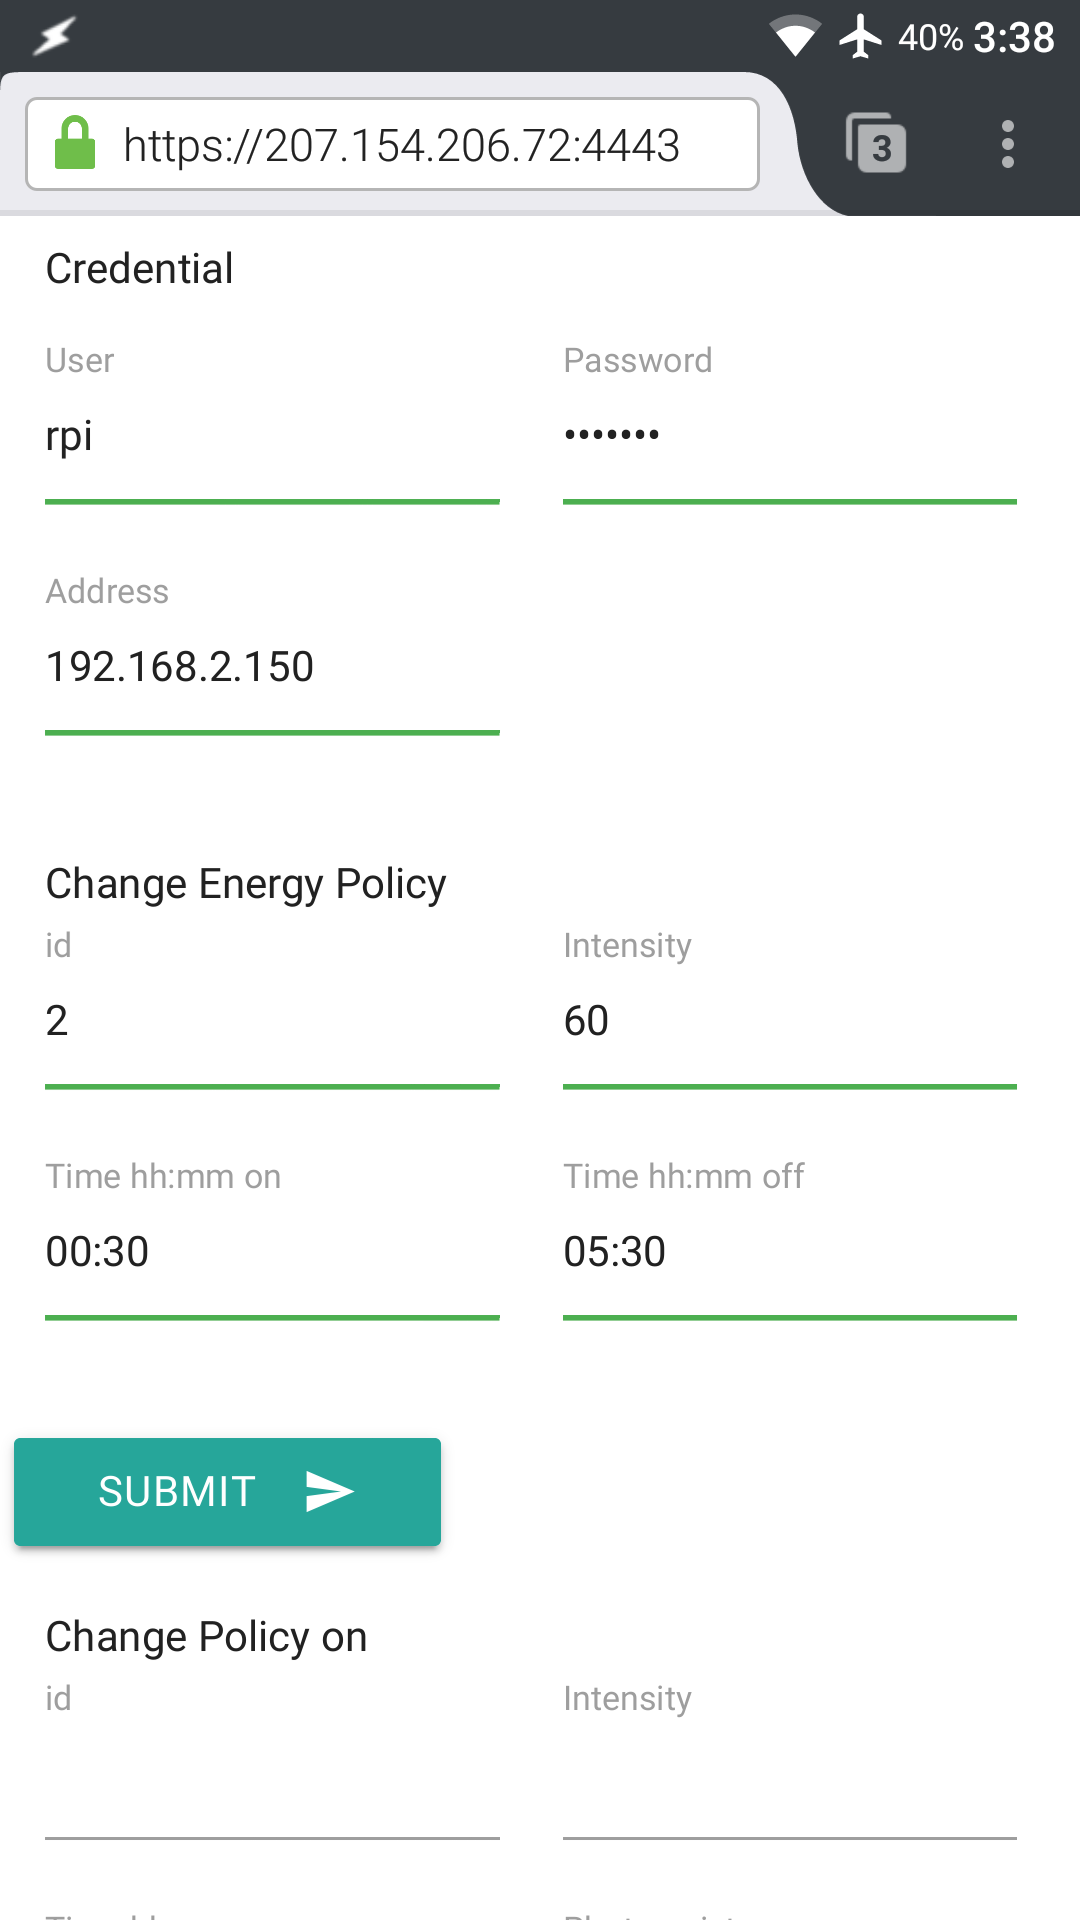
\includegraphics[width=6cm]{figure/web_mobile.png} }}%
	\qquad
	\subfloat[(Mobile) Campi mancanti o errati]{{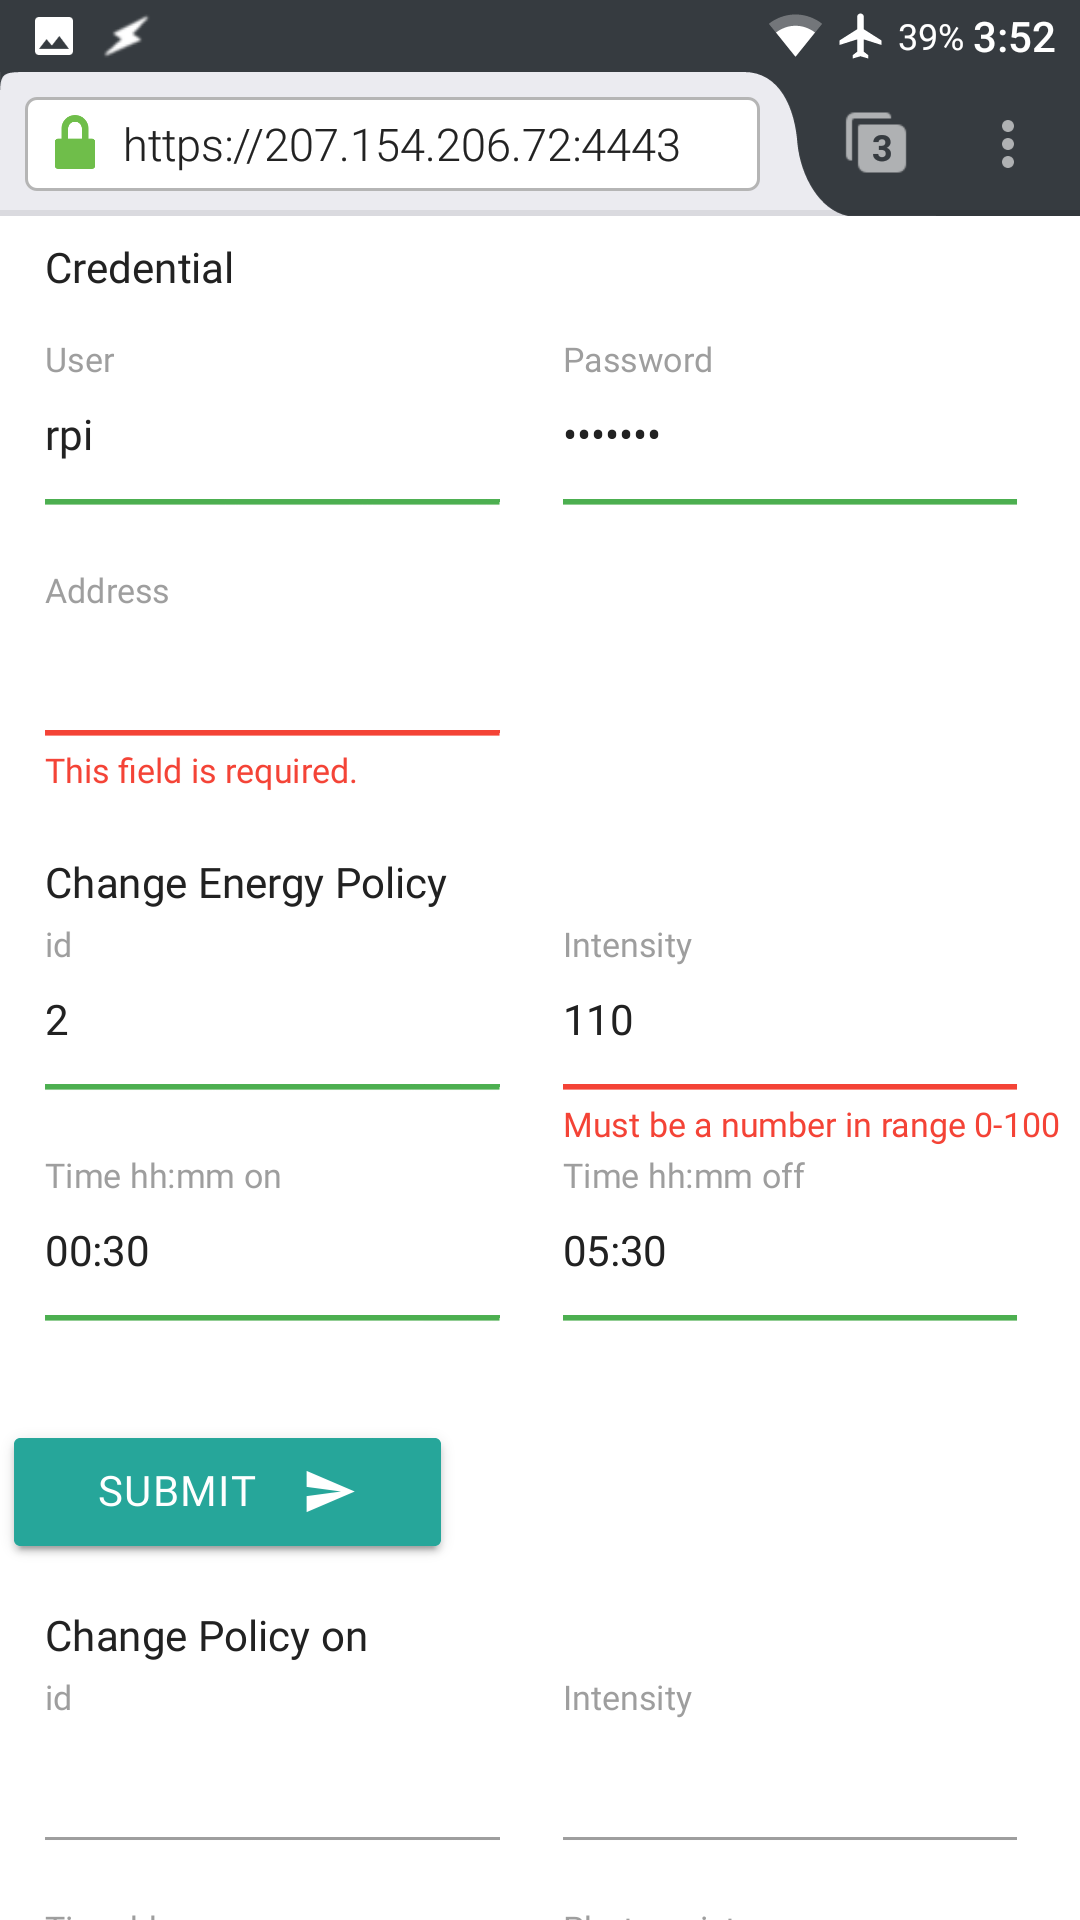
\includegraphics[width=6cm]{figure/web_mobile_errors.png} }}%
	%\caption{Esempi della interfaccia mobile}%
	\label{fig:example}%
\end{figure}

\newpage
\subsection{Linguaggi e librerie}
Nella scelta se realizzare un sito dinamico (con PHP o tecnologie simili) o statico (utilizzando esclusivamente HTML, CSS e Javascript), si è optato per la seconda possibilità, poiché:
\begin{itemize}
 \item il sito consiste in una singola pagina web che contiene sempre le stesse informazioni;
 \item essendo le comunicazioni basate su REST, è il client a contattare direttamente il destinatario, mentre se il sito fosse dinamico, il server fungerebbe da intermediario;
 \item dal punto di vista della sicurezza, evitando di utilizzare PHP si riduce anche la superficie di attacco del server;
 \item essendo il sito piuttosto semplice dal punto di vista delle funzionalità, realizzandolo staticamente è più facile ottenere un design più pulito.
\end{itemize}
Per quanto riguarda lo \textit{style sheet language}, si è valutato di utilizzare direttamente CSS invece di uno strumento di automatizzazione come SASS:
il sito è composto da un'unica pagina Web, di conseguenza uno strumento di come SASS non sarebbe stato di particolare aiuto, e avrebbe inutilmente aggiunto complessità.
Per il CSS si è utilizzata la libreria \textit{materialize}, mentre per quanto riguarda JavaScript sono stati utilizzati \textit{JQuery} e \textit{JQuery validate} (per effettuare controlli client side sui form compilati dagli utenti).




%\chapter*{Ringraziamenti}

%\appendix

\backmatter

\listoffigures
%\bibliography{biblio}
\bibliographystyle{abbrv}

%\listoftables

\end{document}
